\documentclass[border=3pt,tikz,svgnames]{standalone}
\usepackage{tikz}
\usetikzlibrary{decorations.markings,arrows.meta,calc}
\tikzset{>={Stealth[length=1.2mm,width=1.2mm]}}
\colorlet{PurpleFill}{MediumPurple}
\colorlet{PurpleLine}{MediumPurple!30!SlateBlue}

\begin{document}

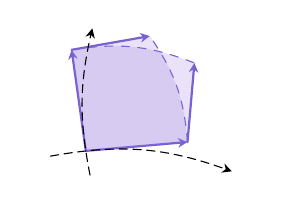
\begin{tikzpicture}[line cap=round]
    \def\Lx{1.44}
    \def\Ly{0.96}
    \path[use as bounding box] (-\Lx,-\Ly) rectangle (\Lx,\Ly);
    \coordinate (O) at (-0.487*\Lx,-0.63*\Ly);
    \coordinate (R) at ($(O)+(98:0.9*\Lx)$);
    \coordinate (Ru) at ($(O)+(98:0.9*\Lx)+(10:0.7*\Lx)$);
    \coordinate (Q) at ($(O)+(5:0.9*\Lx)$);
    \coordinate (Qv) at ($(O)+(5:0.9*\Lx)+(85:0.7*\Lx)$);

    \draw[PurpleLine, thick, ->] (O) -- (R);
    \draw[PurpleLine, thick, ->] (O) -- (Q);
    \draw[PurpleLine, thick, ->] (R) -- (Ru);
    \draw[PurpleLine, thick, ->] (Q) -- (Qv);
    \draw[PurpleLine, dashed, thin] (Q) to[bend right=15] (Ru);
    \draw[PurpleLine, dashed, thin] (R) to[bend left=15] (Qv);

    \fill[PurpleFill, opacity=0.2] (O) -- (Q) to[bend right=15] (Ru) -- (R) -- cycle;
    \fill[PurpleFill, opacity=0.2] (O) -- (R) to[bend left=15] (Qv) -- (Q) -- cycle;

    \draw[densely dashed, thin,->] (-0.45*\Lx,-0.95*\Ly) to[bend left=12] (-0.43*\Lx,0.99*\Ly);
    \draw[densely dashed, thin,->] (-0.8*\Lx,-0.7*\Ly) to[bend left=15] (0.8*\Lx,-0.9*\Ly);
\end{tikzpicture}

\end{document}
